\begin{figure}[H]
	    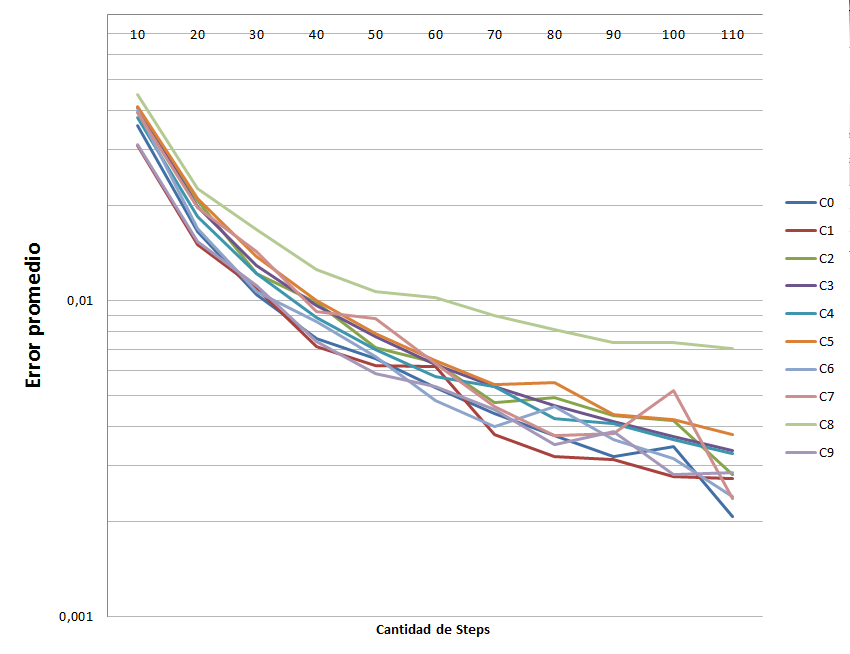
\includegraphics[scale=.60]{imagenes/variacion_parametro_y_columna_steps.png}
	    \caption{Error promedio en Steps para todas las columnas de la tabla brindada por la materia} 
	    \label{fig:variacion_parametro_y_columna_steps}
\end{figure}

	A continuaci\'on, realizamos un an\'alisis del estimador ``Distributed Steps'', el cual obtuvo los mejores resultados seg\'un nuestros analisis previos.
	
	En la figura \ref{fig:variacion_parametro_y_columna_steps} se ve un gr\'afico que se realizo utilizando los errores promedio para cada columna, variando a la ves la cantidad de Steps del estimador. Como error promedio considereamos al promedio de los errores obtenidos para los distintas estimaciones de los valores de una misma columna. Una ves teniendo el error promedio para una cantidad de Steps particular y una columna particular, repetimos el proceso variando la cantidad de Steps para todas las columnas.
	
	Se ve como el error promedio de cada columna, en si es muy similar para pocos Steps, pero al aumentar la cantidad de steps, mejora mucho el error, y esta mejor es, en promedio, independiente de la distribucion de la columna, ya que la diferencia de errores entre columnas, es muy chico.

\begin{figure}[H]
	    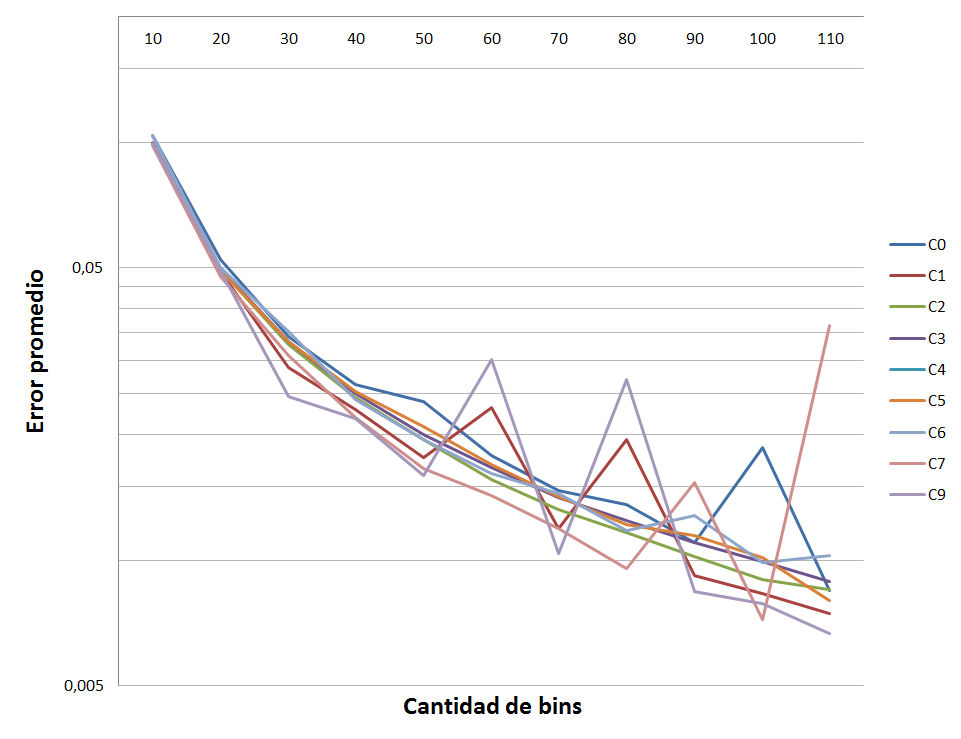
\includegraphics[scale=.60]{imagenes/variacion_parametro_y_columna_histo.png}
	    \caption{Error promedio en Histograma clasico para todas las columnas de la tabla brindada por la materia} 
	    \label{fig:variacion_parametro_y_columna_histo}
\end{figure}

\begin{figure}[H]
	    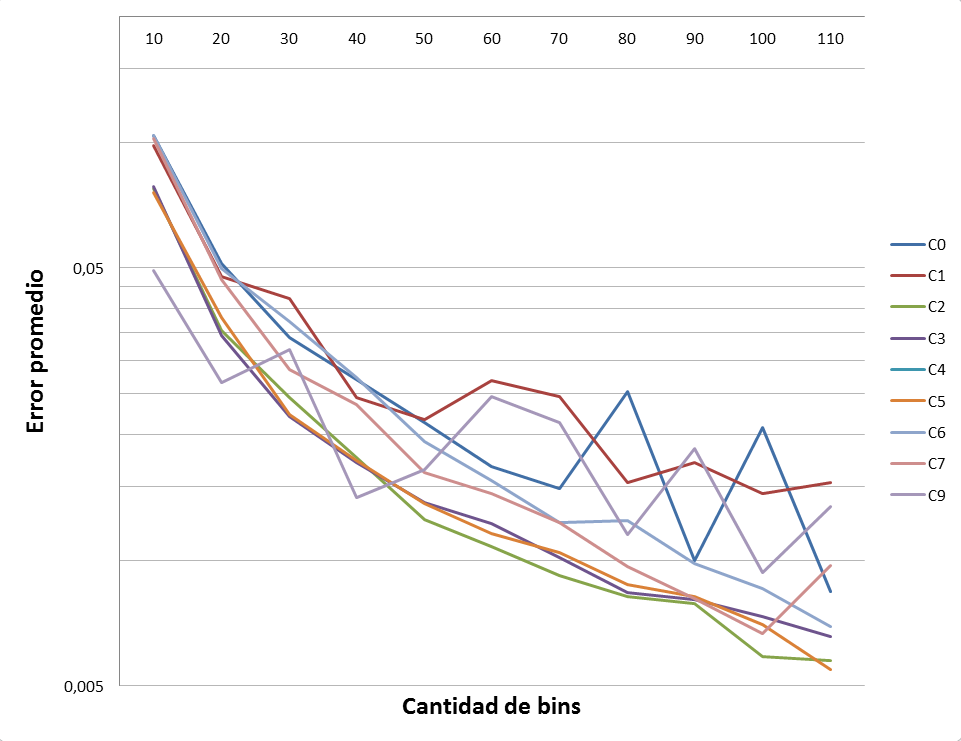
\includegraphics[scale=.60]{imagenes/variacion_parametro_y_columna_grupo.png}
	    \caption{Error promedio en Estimador del grupo para todas las columnas de la tabla brindada por la materia} 
	    \label{fig:variacion_parametro_y_columna_grupo}
\end{figure}

Adicionalmente, se puede ver en las figuras \ref{fig:variacion_parametro_y_columna_histo} y \ref{fig:variacion_parametro_y_columna_grupo} el mismo analisis realizado para Steps, pero esta ves para Histograma clasico y el estimador echo por el grupo respectivamente.

	Comparandolos con el grafico de Steps, a primera vista se ve como en general Steps se comporta mejor un valor del parametro fijo. 
	
	A diferencia de el de steps, el histograma clasico no es tan independiente de la distribucion de los datos, se puede ver como para las distintas columnas el error var\'ia bastante. 
	
	En cuanto al estimador del grupo, lo que se puede apreciar es que para algunas columnas, se comporta mejor que el Histograma cl\'asico, y dificilmente se comporta mejor que Steps. Debido a lo analizado anteriormente, sabemos que el estimador del grupo tenia una mejor performance sobre el cl\'asico solo en las distribuciones normales, y en las uniformes los errores no variaban mucho entre uno y otro. Las columnas donde la performance es mejor que en el histograma, son las C2, C3 y C5. En el anexo a este informe, en la carpeta "/tests/Determinar Distribuciones" se encuentran los gr\'aficos de las columnas mencionadas. No fueron incluidos en este informe, debido a que eran demaciados y nos iban a quedar demaciados gr\'aficos.
	
	En esos gr\'aficos, se puede ver como las distribuciones de esas columnas son todas distribuciones normales, por lo que se puede comprobar que nuestro analisis previo, en donde nuestro estimador se comportaba mejor en distribuciones normales, es correcto.
	